\documentclass{article}[18pt]
\ProvidesPackage{format}
%Page setup
\usepackage[utf8]{inputenc}
\usepackage[margin=0.7in]{geometry}
\usepackage{parselines} 
\usepackage[english]{babel}
\usepackage{fancyhdr}
\usepackage{titlesec}
\hyphenpenalty=10000

\pagestyle{fancy}
\fancyhf{}
\rhead{Sam Robbins}
\rfoot{Page \thepage}

%Characters
\usepackage{amsmath}
\usepackage{amssymb}
\usepackage{gensymb}
\newcommand{\R}{\mathbb{R}}

%Diagrams
\usepackage{pgfplots}
\usepackage{graphicx}
\usepackage{tabularx}
\usepackage{relsize}
\pgfplotsset{width=10cm,compat=1.9}
\usepackage{float}

%Length Setting
\titlespacing\section{0pt}{14pt plus 4pt minus 2pt}{0pt plus 2pt minus 2pt}
\newlength\tindent
\setlength{\tindent}{\parindent}
\setlength{\parindent}{0pt}
\renewcommand{\indent}{\hspace*{\tindent}}

%Programming Font
\usepackage{courier}
\usepackage{listings}
\usepackage{pxfonts}

%Lists
\usepackage{enumerate}
\usepackage{enumitem}

% Networks Macro
\usepackage{tikz}


% Commands for files converted using pandoc
\providecommand{\tightlist}{%
	\setlength{\itemsep}{0pt}\setlength{\parskip}{0pt}}
\usepackage{hyperref}

% Get nice commands for floor and ceil
\usepackage{mathtools}
\DeclarePairedDelimiter{\ceil}{\lceil}{\rceil}
\DeclarePairedDelimiter{\floor}{\lfloor}{\rfloor}

% Allow itemize to go up to 20 levels deep (just change the number if you need more you madman)
\usepackage{enumitem}
\setlistdepth{20}
\renewlist{itemize}{itemize}{20}

% initially, use dots for all levels
\setlist[itemize]{label=$\cdot$}

% customize the first 3 levels
\setlist[itemize,1]{label=\textbullet}
\setlist[itemize,2]{label=--}
\setlist[itemize,3]{label=*}

% Definition and Important Stuff
% Important stuff
\usepackage[framemethod=TikZ]{mdframed}

\newcounter{theo}[section]\setcounter{theo}{0}
\renewcommand{\thetheo}{\arabic{section}.\arabic{theo}}
\newenvironment{important}[1][]{%
	\refstepcounter{theo}%
	\ifstrempty{#1}%
	{\mdfsetup{%
			frametitle={%
				\tikz[baseline=(current bounding box.east),outer sep=0pt]
				\node[anchor=east,rectangle,fill=red!50]
				{\strut Important};}}
	}%
	{\mdfsetup{%
			frametitle={%
				\tikz[baseline=(current bounding box.east),outer sep=0pt]
				\node[anchor=east,rectangle,fill=red!50]
				{\strut Important:~#1};}}%
	}%
	\mdfsetup{innertopmargin=10pt,linecolor=red!50,%
		linewidth=2pt,topline=true,%
		frametitleaboveskip=\dimexpr-\ht\strutbox\relax
	}
	\begin{mdframed}[]\relax%
		\centering
		}{\end{mdframed}}



\newcounter{lem}[section]\setcounter{lem}{0}
\renewcommand{\thelem}{\arabic{section}.\arabic{lem}}
\newenvironment{defin}[1][]{%
	\refstepcounter{lem}%
	\ifstrempty{#1}%
	{\mdfsetup{%
			frametitle={%
				\tikz[baseline=(current bounding box.east),outer sep=0pt]
				\node[anchor=east,rectangle,fill=blue!20]
				{\strut Definition};}}
	}%
	{\mdfsetup{%
			frametitle={%
				\tikz[baseline=(current bounding box.east),outer sep=0pt]
				\node[anchor=east,rectangle,fill=blue!20]
				{\strut Definition:~#1};}}%
	}%
	\mdfsetup{innertopmargin=10pt,linecolor=blue!20,%
		linewidth=2pt,topline=true,%
		frametitleaboveskip=\dimexpr-\ht\strutbox\relax
	}
	\begin{mdframed}[]\relax%
		\centering
		}{\end{mdframed}}
\lhead{Software Methodologies - AI Search}
\lstset{language=Python,
	basicstyle=\ttfamily,
	keywordstyle=\bfseries,
	showstringspaces=false,
	morekeywords={if, else, then, print, end, for, do, while},
	commentstyle=\color{red},
	tabsize=4
}

\begin{document}
\begin{center}
\underline{\huge Heuristic Search}
\end{center}
\section{General Heuristic Search}
\begin{itemize}
	\item We've seen that uniformed search can be extremely expensive
\end{itemize}
\begin{defin}[Heuristic Search (Informed Search)]
	Additional information pertinent to the problem in hand is supplied (or constructed) and used
\end{defin}
We shall continue to base our strategies around the search tree
\begin{defin}[Best-First Search]
\begin{itemize}
	\item Expand a fringe node z with a minimal value according to a given evaluation function $f(z)$
	\begin{itemize}
		\item $f$ is defined on the nodes of the search tree
	\end{itemize}
	\item Put children on the fringe and repeat
\end{itemize}
\end{defin}
Choice of evaluation function determined type of best-first search, e.g.
\begin{itemize}
	\item f(z)="depth of a node" yields a breadth first search
	\item f(z)="1/(depth of a node)" yields a depth first search 
\end{itemize}
In tandem with the choice of termination condition - up until now it has been "stop when a goal node appears on the fringe"
\section{Best-First Search}
\begin{lstlisting}[mathescape=true, tabsize=2]
newid = 1
register node:
S[1]=initial_state;
P[1]=-;
A[1]=-;
PC[1]=0;
D[1]=0;

initialise priority queue (of tuples):
fringe F = [(newid, S[1], P[1], A[1], PC[1], D[1])]
if node 1 is a goal-node then return 1
else
while $F\neq \varnothing$ do:
	pop (id, state, parent_id, action, path_cost, depth) from F
	for each state child and action $\alpha$ for which we have that child $\in$ $\phi$ (state, $\alpha$) do:
		newid=newid+1
		register node:
		S[newid]=child;
		P[newid]=id;
		A[newid]=$\alpha$;
		PC[newid]=PC[id]+$\rho(state, \alpha, child)$;
		D[newid]=D[id]_1;
		if node newid  is a goal node then return newid
		else add (newid, S[newid], P[newid], A[newid], PC[newid], D[newid]) to F
return 0
\end{lstlisting}
\section{Heuristic Functions}
\begin{itemize}
	\item The evaluation function f is usually dependent upon an additional heuristic function, denoted h, where
	\begin{itemize}
		\item $h(z)\geqslant 0$ can be thought of as the estimated cost of the cheapest path in the search tree from node z to any goal-node (recall that all step costs are non-negative)
	\end{itemize}
	\item Every heuristic function must satisfy two constraints
	\begin{itemize}
		\item if z is a goal-node then necessarily h(z)=0 (if you're at the goal node, the cost of getting there is 0)
		\item h(z) only depends upon the state associated with the node z so h(z) is considered as the estimated cost of the cheapest path in the search space from the state associated with z to any goal state
	\end{itemize}
\end{itemize}
\begin{important}[Heuristics]
A heuristic is given as additional information (unless we build it ourselves)\\
The usefulness of a heuristic is almost always dependent upon how good an estimation it is
\end{important}

\section{Greedy best-first search}
\begin{itemize}
	\item The evaluation function equals the heuristic function; that is, f(z)=h(z)
	\item Termination when a goal-node appears on the fringe
\end{itemize}
Consider the following problem:
\begin{itemize}
	\item Initial state: Ashington
	\item Goal state
	\item One action and step costs-shown
	\item Heuristic h is a straight line distance to Bishop Aukland
\end{itemize}
\begin{center}
	\includegraphics[scale=1]{"ashington->bishop aukland"}
\end{center}
The greedy expansion of this doesn't lead to an optimal path
\subsection{Performance of greedy best-first search}
\begin{itemize}
	\item Greedy best-first search need not return an optimal solution
	\begin{itemize}
		\item In fact, greedy best first search need not terminate, i.e. it is incomplete
		\item The diagram below does not complete as Neamt is closest in distance to Fagaras
		\item It keeps looping between Iasi and Neamt
	\end{itemize}
	\item If d is the depth of the shallowest goal-node in the search tree and b is the branching factor then
	\begin{itemize}
		\item In the worst case, the time and space complexity is $\Omega(b^d)$, for the heuristic function could be useless
		\item e.g., h(z)=0 for every z and ties could be broken so that the greedy best-first search proceeds exactly as does BFS
	\end{itemize}
	\item The improvement one gains with greedy best first search is strongly dependent upon the quality of the heuristic function
\end{itemize}
\begin{center}
	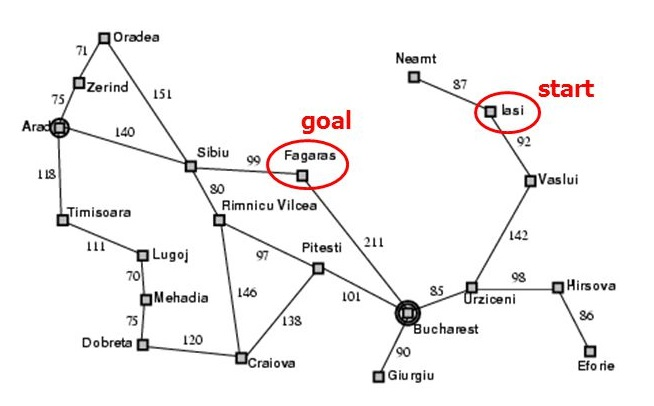
\includegraphics[scale=1]{lasi}
\end{center}
\section{Building a heuristic function}
\begin{itemize}
	\item We can sometimes manufacture our own heuristic function if additional information is not supplied
	\item Consider TSP formulated so that
	\begin{itemize}
		\item States are partial tours $(c_1,c_2,...,c_i)$ i.e., paths where $0\leqslant i\leqslant n$ (where n is the number of cities)
		\item Initial state is the empty partial tour ()
		\item Goal states are the partial tours containing every city, e.g. $(c_1,c_2,...,c_n)$
		\item Transitions are obtained by "visiting an unvisited city" (there is one action)
		\begin{itemize}
			\item $(c_1,c_2,...,c_i)\rightarrow (c_1,c_2,...,c_i,c_{i+1})$ where $c_{i+1}\neq c_j$ for all $j=1,2,..,i$
		\end{itemize}
		\item Step-cost $\sigma((c_1,c_2,..,c_i),(c_1,c_2,...,c_i,c_{i+1}))=\delta(c_i,c_{i+1})$ unless
		\begin{itemize}
			\item $i=n-1$ when $=\delta(c_{n-1},c_n)+\delta(c_n,c_1)$ (loop back to complete tour)
		\end{itemize}
	\end{itemize}
	\item Define the heuristic function $h(z)$ as follows
	\begin{itemize}
		\item If the state associated with tree-node z is $(c_1,c_2,...,c_i)$, where $i\neq n$, then
		$$h(z)=\min\{\delta(c_i,c'): \text{c' is an unvisited city}\}$$
		\item This is the shortest extension you can make to get to an unvisited city from any fringe node
		\item if the state associated with tree-node z is $(c_1,c_2,...,c_n)$ then $h(z)=0$
	\end{itemize}
	\item This heuristic function satisfies the two criteria required for any heuristic function
	\item Our greedy best-first search differs from the "visit-nearest-neighbour" algorithm
	\begin{itemize}
		\item visit-nearest-neighbour goes down, extending from the last extended node
	\end{itemize}
\end{itemize}
\section{A* Search}
\begin{itemize}
	\item The most widely known form of best-first search is A* search
	\begin{itemize}
		\item Evaluates nodes by combining $h(z)$
		\begin{itemize}
			\item The heuristic cost to get from the node z to a goal node and g(z) (g is the sum of the step costs to get to z from the root)
			\item The path-cost (available from the search tree data structure) to reach node z from the root
		\end{itemize}
		\item Evaluation function $f(z)=g(z)+h(z)$
	\end{itemize}
	\item Another way of looking at $f(z)$
	\begin{itemize}
		\item It is the estimated cost of the optimal solution through node z
	\end{itemize}
	\item An A* Search terminates when
	\begin{itemize}
		\item A goal node z is on the fringe and f(z) is minimal amongst fringe nodes
		\begin{itemize}
			\item A* search outputs the path of action from the root to z (of cost f(z)=g(z)) (note that h(z)=0 for a goal node)
		\end{itemize}
		\item or, when there are no nodes to expand. So no goal-node exists, and this is signalled in output
	\end{itemize}
\end{itemize}
\begin{important}[A* Search]
A goal-node is never expanded under A* Search (at that point the heuristic would be 0)\\
A* Search can be both complete and optimal
\end{important}
\end{document}